\subsection{Tools > Projection > Height Grid Generation}

\label{subsection:heightGridGeneration}

\index{projection!sur grille}
\index{grille|see{projection sur grille}}
Cette fonction permet de projeter un nuage de point sur une grille
r�guli�re suivant l'axe Z.\\

\begin{figure}[!h]
\begin{centering}
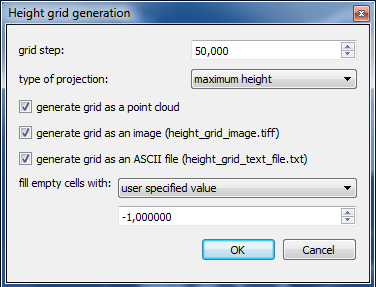
\includegraphics[width=0.45\textwidth]{Partie3_Fonctions/heightGridGenerationDlg.png}
\caption{\label{fig:heightGridGenerationDlg}Interface de param�trage pour
l'outil de projection d'un nuage sur une grille}
\end{centering}
\end{figure}

Une interface (figure~\ref{fig:heightGridGenerationDlg}) permet
de r�gler diff�rents param�tres :
\begin{itemize}
\item \emph{grid step} : le pas de la grille exprim� dans l'unit� des coordonn�es du nuage de points
\item \emph{type of projection} : ce param�tre peut prendre l'une des 2
valeurs suivantes :

\begin{itemize}
\item \textit{maximum height} : soit E$_{ij}$ le sous-ensemble de points du nuage
qui est projet� dans la case (i,j) de la grille. Pour chaque case (i,j)
de la grille, on retient comme altitude Z celle du point le plus haut
dans E$_{ij}$.
\item \textit{average height} : pour chaque case (i,j) de la grille, on
retient comme altitude Z l'altitude moyenne des points de E$_{ij}$.
\end{itemize}
\item \emph{fill empty cells with} : certaines cases de la grille r�guli�re
restent vides apr�s projection (aucun point du nuage ne s'y projette).
Ce param�tre indique avec quelle valeur l'on doit renseigner ces cases et peut prendre l'une des 3 valeurs suivantes :

\begin{itemize}
\item \textit{minimum height :} les cases vides sont renseign�es avec l'altitude
Z minimale parmi tous les points du nuage.
\item \textit{average height} : les cases vides sont renseign�es avec l'altitude
Z moyenne de tous les points du nuage.
\item \textit{maximum height} : les cases vides sont renseign�es avec l'altitude
Z maximale parmi tous les points du nuage.\\
\end{itemize}
\end{itemize}
\par
Cette fonction g�n�re deux fichiers (dans le r�pertoire du binaire
de \emph{CloudCompare} par d�faut) :
\begin{itemize}
\item \emph{height\_grid\_image.tiff} : l'image raster 2D cod�e sur 256 niveaux
de gris correspondant aux altitudes Z des points projet�s dans les cases de la grille ;
\item \emph{height\_grid\_text\_file.txt} : les donn�es de la grille sous un format ASCII (fichier exploitable
simplement par un programme).\\
\end{itemize}
\par
Voir figure~\ref{fig:heightGridGenerationExample} pour exemple de r�sultat produit par cette fonction.

\begin{figure}[!htb]
\begin{centering}
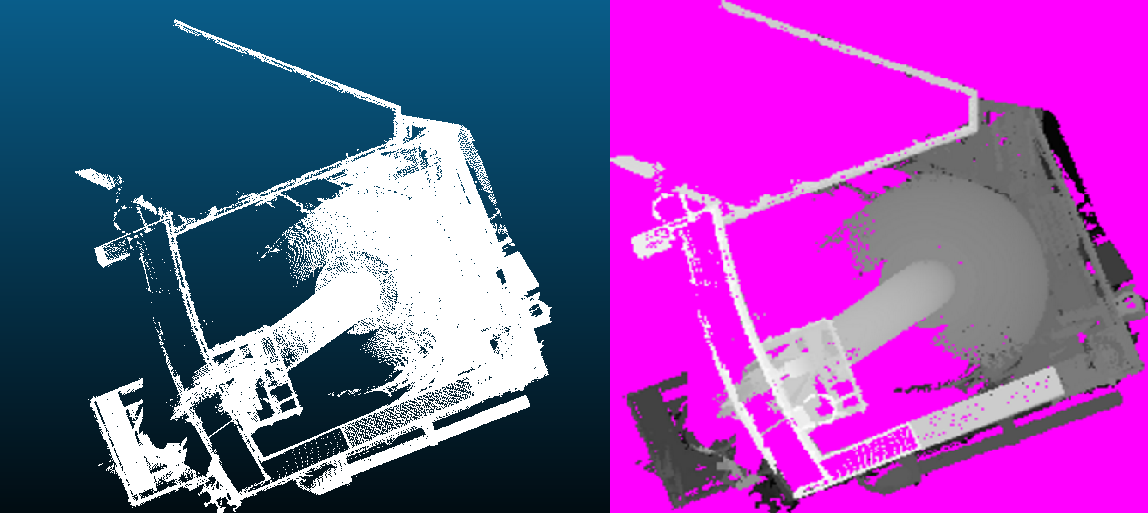
\includegraphics[width=0.95\textwidth]{Partie3_Fonctions/HeightGridImageExample.jpg}
\par\end{centering}
\caption{\label{fig:heightGridGenerationExample}Exemple de r�sultat : vue 3D � gauche, image 2D des hauteurs � droite}
\end{figure}
